\subsection{Внутритекстовые и выключные формулы}

Небольшие математические выражения включаются непосредственно в предложение.
Например, условная система искусственного интеллекта может оценивать уверенность в ответе числом $q \in \seg{0}{1}$.
Если формула играет самостоятельную роль или содержит длинное выражение, её целесообразно вынести на отдельную строку.

Пусть $p$~--- число правильно решённых задач, $c$~--- число проверенных ссылок, а $h$~--- число обнаруженных галлюцинаций.
Введём условный рейтинг системы:
\begin{equation}\label{eq:рейтинг_системы}
    R \is 2p + c - 3h.
\end{equation}
Формула~\eqref{eq:рейтинг_системы} будет использоваться в следующей главе.

Ненумерованная выключная формула оформляется окружением \verb|equation*|:
\begin{equation*}
    R = 2 \mul 7 + 4 - 3 \mul 2 = 12.
\end{equation*}

Для переноса длинного выражения используется окружение \verb|split|:
\begin{equation*}
    \begin{split}
        S
            & = a_1 + a_2 + a_3 + {} \\
            & + a_4 + a_5 + a_6.
    \end{split}
\end{equation*}
Знак сложения сохраняется в конце первой строки и повторяется в начале второй.

Для цепочки преобразований с пояснениями справа используется окружение \verb|aligned|:
\begin{equation*}
    \begin{aligned}
        R
            & = 2p + c - 3h
                && \text{(определение рейтинга)} \\
            & = 2 \mul 7 + 4 - 3 \mul 2
                && \text{(подстановка значений)} \\
            & = 12.
                && \text{(результат)}
    \end{aligned}
\end{equation*}

Кусочно-заданное правило оформляется окружением \verb|cases|.
Например, решение автоматического проверяющего модуля можно задать следующим образом:
\begin{equation*}
    D(R, h) \is
    \begin{cases}
        1, & R \ge 10 \land h = 0, \\
        0, & R < 10 \lor h > 0.
    \end{cases}
\end{equation*}


\subsection{Именованные ссылки на блоки}

\begin{table}[t!]
    \caption{Результаты условной проверки трёх систем искусственного интеллекта.}
    \label{tbl:результаты_систем}
    \centering
    \begin{tabular}{|c|c|c|c|c|}
        \hline
        Система & $p$ & $c$ & $h$ & $R$ \\
        \hline
        A-17 & 1 & 2 & 2 & $-2$ \\
        \hline
        B-42 & 3 & 4 & 0 & 10 \\
        \hline
        C-314 & 5 & 3 & 1 & 10 \\
        \hline
    \end{tabular}
\end{table}

Для ссылки на нумерованный семантический блок используется команда \verb|\blink|.
Например, понятие высказывания было введено в \blink{определении высказывания}{defi:высказывание}.
Название объекта передаётся в первом аргументе в той грамматической форме, которая требуется предложением.
Второй аргумент содержит метку объекта.
Для ссылки на формулу применяется команда \verb|\eqref|.
Так, рейтинг системы определяется формулой~\eqref{eq:рейтинг_системы}.
Для рисунков и таблиц снова используется команда \verb|\blink|.
Например, см.~\blink{табл.}{tbl:результаты_систем}.

\subsection{Демонстрация вставки рисунка}

Рассмотрим правила де~Моргана для операций над множествами.

\stat{stat:правила_де_моргана_для_множеств}
{Правила де~Моргана для множеств}{
    Для любых множеств $A, B \subset M$ выполнены равенства
    \begin{equation*}
        \begin{aligned}
            M \setminus (A \cup B)
                & = (M \setminus A) \cap (M \setminus B), \\
            M \setminus (A \cap B)
                & = (M \setminus A) \cup (M \setminus B).
        \end{aligned}
    \end{equation*}
}[
    Докажем первое равенство.
    Для произвольного $x \in M$ имеем:
    \begin{equation*}
        \begin{aligned}
            x \in M \setminus (A \cup B) \eq
                & \eq x \not\in A \cup B \eq \\
                & \eq (x \not\in A) \land (x \not\in B) \eq \\
                & \eq x \in (M \setminus A) \cap (M \setminus B).
        \end{aligned}
    \end{equation*}
    Следовательно, множества в левой и правой частях первого равенства состоят из одних и тех же элементов.
    Второе равенство доказывается аналогично с использованием логического равенства $\lnot (P \land Q) \eq (\lnot P \lor \lnot Q)$.
]

\begin{figure}[t!]
    \centering
    \begin{subfigure}[b]{.45\textwidth}
        \centering
        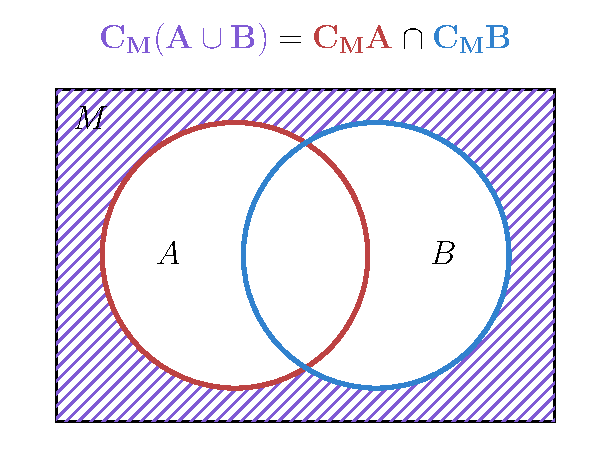
\includegraphics[scale=0.58]{l-01/demorgan_union.pdf}
    \end{subfigure}
    \hfill
    \begin{subfigure}[b]{.45\textwidth}
        \centering
        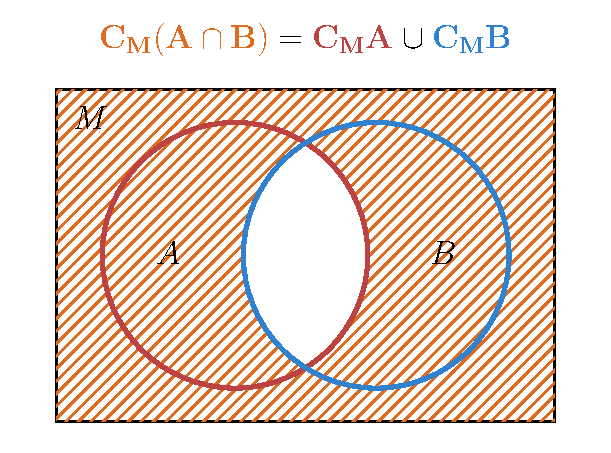
\includegraphics[scale=0.58]{l-01/demorgan_intersection.pdf}
    \end{subfigure}
    \caption{Иллюстрация правил де~Моргана для объединения и пересечения множеств.}
    \label{fig:правила_де_моргана}
\end{figure}

Сформулированные в \blink{утверждении о правилах де~Моргана}{stat:правила_де_моргана_для_множеств} равенства наглядно проиллюстрированы на \blink{рис.}{fig:правила_де_моргана}.